\documentclass{amia}
\usepackage{graphicx}
\usepackage[labelfont=bf]{caption}
\usepackage[superscript,nomove]{cite}
\usepackage{color}
\usepackage{multirow}


\begin{document}


\title{Designing an effective intervention of motivational interview using sequence classification methods}

\author{Mehedi Hasan, BS$^{1}$, Alexander Kotov, PhD$^{1}$, April Carcone, PhD$^{2}$, Sylvie Naar-King, PhD$^{2}$}

\institutes{
$^1$Department of Computer Science,  
$^2$Pediatric Prevention Research Center, Wayne State University, Detroit, Michigan\\
}

\maketitle

\noindent{\bf Abstract}
\textit{Childhood obesity is a serious public health concern in the United States and worldwide. Therefore, there is a need for identification of successful and unsuccessful motivational interviews to facilitate the development of effective interventions for childhood obesity. This paper describes our work on the classification of utterance sequences to distinguish different behavior outcomes such as positive change talk or commitment versus negative change talk or commitment. Markov chain and hidden Markov models were employed and compared with a different order for the classification of utterance sequences. The classification performances achieved 75.32\% and 79.89\% F-measure for normal sequences and 97.36\% and 96.99\% F-measure for alternate sequences using 1st order Markov chain and second order hidden Markov model, respectively. }

\section*{Introduction}
In the recent times, more and more data from various domains being produced in the form of event sequences. Thus, sequence classification has become an important task in sequence mining. Sequences can contain discrete (e.g., symbolic sequences such as text, proteins, or DNA) or continuous events (e..g, time series such as ECGs or stocks), depending on the event types. Usually, sequences don't have explicit features and suffer with high dimension of feature space. Even the sequential nature of features is too difficult to capture, which make sequence classification, a more challenging task than feature-based classifications. The sequence classification methods can be divided into three large categories: feature-based classification, distance based method and model based classifications. In feature-based classification, a sequence is transformed into a single vector of features. A supervised learning algorithm such as an support vector machine \cite{leslie2004fast} or decision tree \cite{chuzhanova1998feature} can be used to train the classifier. An improvement of feature-based classifier such as shapelet \cite{ye2009time} or pattern-based \cite{kudenko1998feature, lesh1999mining} approach is used for sequence classifications. On the other hand, distance based method measure the similarity between sequences to determine the quality of the classification significance. The most commonly used distance function is euclidian distance \cite{keogh2003need}, while Dynamic Time Wrapping \cite{keogh2000scaling} is used when more flexible matching is desired in time series data. The third category of sequence classification is model based classifiers such as Hidden Markov Model \cite{rabiner1989tutorial} (HMM) or other statistical models. Recently, a hierarchical approach \cite{nallam2016effective} is proposed for sequence classification. 

Sequence classification has a broad range of real word applications such as information retrieval, genomic analysis, health informatics, finance and abnormal detection. In genomic research, sequence classification is widely used to detect the function of a new protein \cite{deshpande2002evaluation}. In health informatics, ECG can be used as a multi-dimensional time series data to classify an individual as healthy or patient with heart disease \cite{wei2006semi}. Another example is to classify rumour stance in Twitter \cite{lukasik2016hawkes}. In information retrieval, sequence classification is employed to build  models for classifying documents into different topic categories \cite{sebastiani2002machine} such as sports, politics, news, finance and style. Sequence classification is also used in anomaly detection such as abnormal access to systems \cite{lane1999temporal}, malware detection \cite{drew2017polymorphic} and money laundering \cite{liu2008sequence}. Other interesting applications include classifying query log sequences to distinguish web-robots from human users \cite{duskin2009distinguishing, tan2004discovery}. In computer vision, sequence classification is applied for classifying images \cite{li2000image} and videos \cite{zhang2016tensor}.    

In this paper, our target area of application is motivational interview. In particular, this paper describes our work on the classification of utterance sequences. Classification of utterance sequences to distinguish different behavior outcomes such as positive change talk or commitment verses negative change talk or commitment, is an important part of clinical research aimed at designing effective interventions for many conditions and disorders. In this study, we focus on the transcripts of Motivational Interviews with obese adolescents (teens) and their caregivers. Childhood obesity is a serious public health concern in the United States and worldwide. Recent estimates indicate that approximately one third (31.8\%) of US children age 2-19 years are overweight and 16.9\% are obese \cite{ogden2012prevalence}. Adolescents who are obese are likely continue to be obese in adulthood and have a greater risk of heart disease, type 2 diabetes, stroke, cancer, and osteoarthritis \cite{general2010surgeon}. Therefore, there is a need for informatics-based methods to facilitate development of effective interventions for childhood obesity. One approach to designing an effective intervention is Motivational Interviewing (MI), an evidence-based counseling technique to increase intrinsic motivation and self-efficacy for health-related behavior change. The goal of a MI counseling session is to encourage patients to explore their own desires, ability, reasons, need for and commitment to the targeted behavior change. These statements, referred to as ``change talk'' (or CT), consistently predict actual behavior change that can be sustained for as long as 34 months after an interview. 

Our previous studies \cite{kotov2015interpretable, hasan2016study} explored several machine learning methods for the automatic annotation of clinical interview fragments, which uses a codebook \cite{carcone2013provider} with 115 different behavior codes. In this study, probabilistic models are employed for the analysis of sequence data to determine provider-patient communication sequences that are likely to translate into change talk and commitment language. To the best of our knowledge, there have been very limited studies on sequence classification in motivational interview such as patient-provider dialogue. A sequential analysis \cite{eide2004physician} was performed on physician-patient dialogue to find the relationship between physician and patient behaviors associated with patients' exibiting cues. Currently, a very similar work \cite{jaber2016multi} was done on education data, where a sequence classification model was developed to predict the role of a student in a project team based on their communication patterns. Although Hidden Markov Model was originally applied to speech recognition \cite{rabiner1989tutorial}, this is one of the most successful method \cite{mutsam2016maximum, eickeler1998hidden, srivastava2007hmm, won2004training, chai2001folk} for sequence classification. In addition, a k-order Markov Model is applied on genomic research \cite{yakhnenko2005discriminatively} to classify protein and text sequence data.  Therefore, we utilize Markov Chain and Hidden Markov Model for the classification of utterance sequences.   

\section*{Methods}
\subsection*{\textit{Data collection}}
The experimental datasets for this work were constructed based on the transcripts of 37 motivational interview sessions, which include a total of 11,353 segmented and annotated utterances. A fragment of an adolescent session transcript is presented in Table~\ref{table:anno_examp}. The utterances were annotated based on MYSCOPE codebook \cite{carcone2013provider} with 115 different behavior codes, which are grouped into the youth, caregiver, and counselor code groups. These utterances are then scanned from first to last and divided into successful and unsuccessful sequences when a commitment or change talk is found. A total of 1072 sequences have been observed which further partitioned into two subsets based on the outcome of motivational interviews: one dataset that includes all sequences of positive change talk or commitment language (882 sequences) and the other dataset which includes utterances ended with negative change talk or commitment language (192 sequences). In our experiment, these two subsets are utilized to train two Markov chain or HMM.\\

\begin{table*}[htb]
\caption{Fragment of the annotated transcript of a dialogue between a counselor and an adolescent.}    
\label{table:anno_examp}
\centering
\begin{tabular}{lp{3.6cm}lp{8cm}}
\hline
\hline
Annotation  & Description & Speaker & Text \\
\hline
331 &	Open-ended question, elicit change talk positive &	Counselor &	do you feel like making healthier choices for your snacks and your meals is something you would be able to do ? mm-hmm meaning is that food available for you ? \\
117 &	Low Uptake, positive	& Adolescent &	Yes \\
301 &	Structure Session	& Counselor &	okay and thats an important thing for us to think about cause i would not want to help you come up with a plan that you would not be able to do without somebody else help so the last part of your plan is how somebody could be supportive to you meaning how they can help you be successful and so we should choose somebody who you feel like is around often enough \\
112 &	Change Talk positive	& Adolescent &	my um aunt \\
301 &	Structure Session	& Counselor &	okay so lets stick something my aunt can do \\
112 &	Change Talk positive &	Adolescent &	she could when i am doing when i am eating something that i should i could not be eating but so i can choose something healthy she could tell me not to eat it \\
309 &	Affirm, low &	Counselor &	okay that sounds like a really great suggestion \\
\hline
\hline
\end{tabular}
\end{table*}

\subsection*{\textit{Sequence classification techniques}}
Generally, a sequence is an ordered list of events. In our study, event is a behavior code represented as a symbolic value such as 117 (low uptake, positive), 331 (open-ended question), etc.  Given a sequence of behavior codes represented as $S_i = \{x_1, x_2,...,x_n\}$ and a set of class labels $L = \{l_1, l_2,...,l_m\}$, the task of sequence classification is to learn a sequence classifier C, which is a function mapping a sequence $S_i$ to a class label $l_i \in L$, written as, $C : S_i \to l_i, l_i \in L$. Here, L is fixed and known in advances. In our experiment, known labels are ``successful'' and ``unsuccessful'' motivational interview. 

\textbf {Markov Chain}: In probability theory, a markov model \cite{} is a stochastic model used to model randomly changing systems where it is assumed that future states depend only on the present state and not on the sequence of events that preceded it (that is, it assumes the markov property). Generally, this assumption enables reasoning and computation with the model that would otherwise be intractable. For the sequential analysis, we built two markov models $M$ and $\overline{M}$ describing provider strategies and patient responses in case of successful ($M$) and unsuccessful ($\overline{M}$) motivational interviews. A markov model $M$ can be represented as a weighted directed graph $G = (V, E, p)$, in which:

\begin{itemize}
\item $V = \{CML+, CHT+, CHT-, T-AMB, CCT, BLT, LUP+, LUP-, HUP-W, ...\}$ is a set of vertices, consisting of possible youth and counselor MI behavior codes;
\item $E \subseteq V \times V$ is a set of edges corresponding to posssible transitions from one MI behavior code to the other in a sequence;
\item $p_M:E\rightarrow[0...1]$ is a function that assigns probability $p(c_i|c_j)$ to an edge between the MI behavior codes $c_i$ and $c_j$ based on maximum likelihood estimator:

\begin{equation}
P_M(c_j|c_i) = \frac{n_{c_i,c_j}}{n_{c_i}}
\end{equation}

\end{itemize}

where $n_{c_i,c_j}$ and $n_{c_i}$ are the number of times a transition between the MI behavior codes $c_i$ and $c_j$ and the code $c_i$ have been observed in the training data. Given a markov model $M$ (such that $S\subseteq V$), a sequence of MI behavior codes $S = \{C_1,...,C_N\}$ have been generated from a markov model $M$ is:

\begin{equation}
P_M(S) = \prod_{i=2}^N p_M(c_i|c_1,\dots,c_{i-1})=\prod_{i=2}^N p_M(c_i|c_{i-1})
\end{equation}

Success of a given motivational interview, given a sequence of MI behavior codes corresponding to it, can be predicted based on the following formula:

\begin{equation}
p(S\rightarrow CT) = \log\left(\frac{P_M(S)}{P_{\overline M}(S)}\right)= \sum_{i=2}^N p_M(c_i|c_{i-1})-\sum_{i=2}^N p_{\overline M}(c_i|c_{i-1})
\end{equation}

if $p(S\rightarrow CT) > \delta $, where $\delta$ is experimentally defined threshold, the interview transcript (or a portion of it) is predicted to result in CT. We experimentally determined the value of $\delta$ to 0.3 which provides acceptable accuracy with minimum false positive rate. Figure\ref{fig:delta} illustrates the characteristics of proposed model by varying the value of $\delta$. 

The Markov Model we have discussed so far is referred to as the first order Markov Model, since we only look one code in the past to compute the transition probability. A generalization of the first order markov model is the $k^{th}$ order markov chain in which the transition probability for a particular symbol $x_i$ is computed by looking at the k preceding symbols. Thus, $k^{th}$ order markov chain will have $N^{k}$ states each associated with a sequence of k symbols. In our experiment, we also used second order markov model. Hence, our model have $N^2$ states with transitional probability matrix of size $N^2 \times N$.  

\textbf {Hidden Markov Model}: Hidden Markov Models are widely used for sequence analysis because of their ability to incorporate dependencies among elements in sequence. HMM (Hidden Markov Model) is a very
powerful tool to statistically model a process that varies in time. It can be seen as a doubly embedded stochastic process with a process that is not observable (hidden process) and can only be observed through another stochastic process (observable process) that produces the time set of observations. A HMM can be fully specified by (1) N, the number of states in the model; (2) M, the number of distinct observation symbols per state; (3) { } A ij = a , the state transition probability distribution; (4) { ( )} B j = b k , the observation symbol probability distribution; and (5) { } Π = π i , the initial state distribution[10]. The Baum-Welch reestimation method was implemented to train a hidden Markov model for each country using the training set. To identify the country of an unknown melody, the Viterbi algorithm was used to decode the sequence and compute its log probabilities respectively using HMM’s trained for different countries. We then assign the melody to the country with the highest log probability.  

\subsection*{\textit{Evaluation methods}}
To ensure the robustness of performance estimates, we used 10-fold cross validation for the annotation of clinical interview fragments, and 5-fold cross validation for the classification of sequence of behavior codes \cite{} as an experimental design. The performance of different classifiers and feature sets was evaluated in terms of precision, recall, F1 score (F1), kappa measure and accuracy using weighted macro-averaging over folds.

\section*{Results}
Experimental evaluation of automatic annotation of clinical interview fragments and their sequences by using machine learning and probabilistic model included several dimensions:
\begin{itemize}
\item determining the performance of classifiers on the codebooks of different size;
\item determining the effectiveness of the proposed contextual and semantic features.
\item determining the performance of markov model in conjunction with determining PPC sequences that are most likely to translate into CT.
\end{itemize}

Since clinical researchers typically annotate caregiver and adolescent sessions separately, we first created two experimental datasets consisting of only adolescent and only caregiver session transcripts. Second, besides evaluating the accuracy of annotating adolescent and caregiver transcripts with the codebooks containing an entire set of codes, we also conducted a series of experiments with the codebooks of smaller sizes created as outlined above. Third, besides training and testing NB, SVM, CRF, Decision Tree, Boosting, DiscLDA, Random Forest and CNN classifiers using only lexical features, we also evaluated the effectiveness of the proposed contextual and semantic features.

\begin{figure}[htb!]
    \centering
    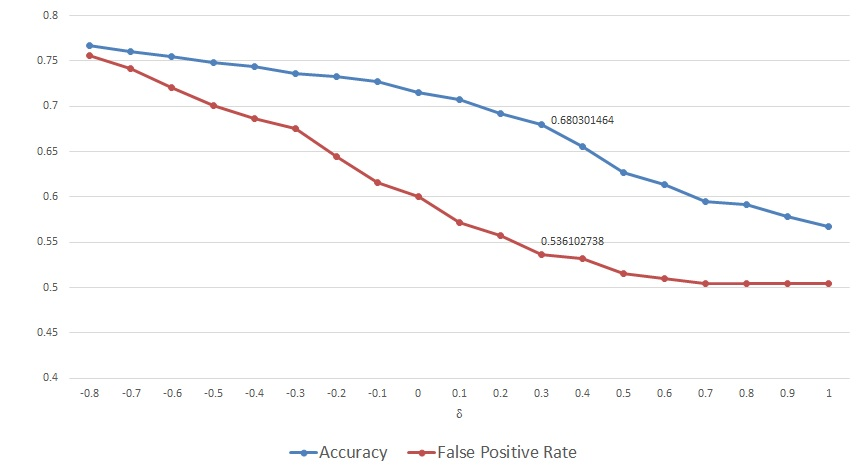
\includegraphics[width=0.70\textwidth]{figures/deltadata.png}
    \caption{\textbf{Characteristics of proposed markov model by varying the value of $\delta$}}
    \label{fig:delta}
\end{figure}

Depending on the type of the interview transcript and the codebook size, SVM-AF achieves 3\%--9\% higher accuracy and 4\%--10\% higher F1 score than SVM and 4\%--10\% higher accuracy and 4\%--11\% higher F1 score than CRF, which highlights the importance of contextual and semantic features. 

\subsection*{\textit{Performance of Markov model in conjunction with determining PPC code sequences that are most likely translate into CT}}
Since clinical researchers tried to increase the desire and ability of adolescent to change their current behavior to target behavior, we used sequence of successful and unsuccessful codes only from adolescent session for our sequential analysis. Summary of performance for the classification of sequential data is presented in Table~\ref{table:sequence}. From Table~\ref{table:sequence}, it follows that our designed markov model works very well in terms of precision and achieves precision 0.7574 with F1-measure 0.7092. The strength of the model for the classification of each type of sequences is illustrated by providing the confusion matrix in Table~\ref{table:conf}. It also shows that successful patterns are identified more accurately compare to unsuccessful motivational interview sequences due to the imbalance of data.\\

\begin{table}[h]
\centering
\caption{Performance of markov models for the classification of normal PPC code sequence.}
\label{tab:result_norm_seq}
  \begin{tabular}{|l|l|l|l|l|l|}
  \hline
   \textbf{Model} & \textbf{Order}  & \textbf{Precision}  & \textbf{Recall} & \textbf{F-Measure} & \textbf{Accuracy}\\ \hline    
    
 \multirow{2}{*}{General Markov Chain} & First order & 0.7387 & 0.7686 & 0.7532 & 0.7686\\\cline{2-6}
 & Second order & 0.6889 & 0.7889 & 0.7352 & 0.7889\\ \hline
 \multirow{2}{*}{Hidden Markov Model} & First order & \textbf{0.7980} & 0.8059 & \textbf{0.7989} & 0.8059\\ \cline{2-6}
 & Second order & 0.7400 & \textbf{0.8449} & 0.7822  & \textbf{0.8449}\\ \hline
 
  \end{tabular}
\end{table}

Two markov models are used to obtain top five most likely successful and unsuccessful motivational interviews that describing provider strategies and patient responses. Table~\ref{table:topsec} shows the top five successful and unsuccessful PPC code sequences.

In general, these higher order models have better classification accuracy as compared to lower order models because they are able to capture longer ordering constraints present in the dataset. However, the number of states in higher order Markov chains grows exponentially with the order of the chain. Consequently, it is harder to accurately estimate all the transition probabilities from the training set. That is, there are many high-order states that are not frequently observed in the training set, leading to inaccurate probability estimates. In principle, this problem can be solved if the size of the training set is increased at the same rate as the state-size of the higher order Markov chain. However, this cannot be easily done for many applications areas. To overcome these problems many variants of the Markov chains have been developed. In the next section we discuss two such variants: the Interpolated Markov Models [SDKW98] and the Selective Markov Models [DK01]. The basic idea of these approaches is to combine portions of different order Markov chains so that to improve the overall classification accuracy.\\

\begin{table}[h]
\centering
\caption{Performance of markov models for the classification of alternate PPC code sequence.}
\label{tab:result_alt_seq}
  \begin{tabular}{|l|l|l|l|l|l|}
  \hline
   \textbf{Model} & \textbf{Order}  & \textbf{Precision}  & \textbf{Recall} & \textbf{F-Measure} & \textbf{Accuracy}\\ \hline    
    
 \multirow{2}{*}{General Markov Chain} & First order & 0.9777 & 0.9437 & 0.9604 & 0.9437\\\cline{2-6}
 & Second order & \textbf{0.9778} & 0.9694 & \textbf{0.9736} & 0.9694\\ \hline
 \multirow{2}{*}{Hidden Markov Model} & First order & 0.9392 & 0.9313 & 0.9253 & 0.9392\\ \cline{2-6}
 & Second order & 0.9704 & \textbf{0.9713} & 0.9699  & \textbf{0.9713}\\ \hline
 
  \end{tabular}
\end{table}

\section*{Discussion}
From the sequential analysis, we observed that markov model achieved near-human accuracy to categorise the sequence of behavior codes. It was also found that successful interviews are more frequently responded by the adolescent with PPC code 112. However, unsuccessful interviews are responded with the behavior code 109.

\section*{Conclusion}
It has been shown how Hidden Markov Models could be used to build classifiers for the sequence of behavior codes in motivational interviews. In this work, we suggest some successful sequences of codes for the practical use by the clinician during the interview session which will translate into positive change talk and commitment language. This work can facilitate researchers to establish causal relationship between different communication strategies and desired behavioral outcomes without having to repeatedly wade through pages of interview transcripts. Information that can directly inform and increase the efficiency of clinical practice for a successful interview. Direction of future work include the exploration of other methods such as BLAST \cite{altschul1990basic} and Strand \cite{drew2014strand} for the classification of utterance sequences. 


\section*{Acknowledgments}
We would like to thank the technical staff at Pediatric Prevention Research Center and Textual Data Analytics Laboratory at Wayne State University for their help with collecting and transforming data into free text EHR used for experiments reported in this paper. 

\bibliographystyle{vancouver}
\bibliography{references}

\end{document}